% Copyright (c) 2021 Eclipse Arrowhead Project
%
% This program and the accompanying materials are made available under the
% terms of the Eclipse Public License 2.0 which is available at
% http://www.eclipse.org/legal/epl-2.0.
%
% SPDX-License-Identifier: EPL-2.0

With the major themes of the \GlossaryHyperRef{framework-arrowhead}{Arrowhead framework} now established, we proceed to outline its most significant concepts in detail.
Each subsection of this section \GlossaryHyperRef{description}{describes} one of these concepts, which are as follows:

\vfill

\noindent\begin{tabularx}{\textwidth}{@{} p{0.9cm} p{4.3cm} X @{}}

\ref{sec:concepts:stakeholder} & \textbf{\nameref{sec:concepts:stakeholder}} & A person or \GlossaryHyperRef{organization}{organization} engaged in an \GlossaryHyperRef{entity}{entity} or undertaking. \\
\ref{sec:concepts:entity}      & \textbf{\nameref{sec:concepts:entity}}      & An \GlossaryHyperRef{artifact}{artifact} that can be distinguished from all other artifacts. \\
\ref{sec:concepts:device}      & \textbf{\nameref{sec:concepts:device}}      & A physical \GlossaryHyperRef{entity}{entity} with the \GlossaryHyperRef{capability}{capability} of hosting \GlossaryHyperRef{system}{systems}. \\
\ref{sec:concepts:system}      & \textbf{\nameref{sec:concepts:system}}      & A \GlossaryHyperRef{instance-software}{software instance} able to exercise the \GlossaryHyperRef{capability}{capabilities} of its hosting \GlossaryHyperRef{device}{device}. \\
\ref{sec:concepts:service}     & \textbf{\nameref{sec:concepts:service}}     & A set of \GlossaryHyperRef{operation}{operations} \GlossaryHyperRef{provider-service}{provided} by a \GlossaryHyperRef{system}{system} for other systems to \GlossaryHyperRef{consumer-service}{consume}. \\
\ref{sec:concepts:sos}         & \textbf{\nameref{sec:concepts:sos}}         & A set of \GlossaryHyperRef{system}{systems} that jointly facilitate new \GlossaryHyperRef{capability-system}{capabilities}. \\
\ref{sec:concepts:local-cloud} & \textbf{\nameref{sec:concepts:local-cloud}} & A \GlossaryHyperRef{cloud}{cloud} with a \GlossaryHyperRef{boundary-local}{local boundary} and \GlossaryHyperRef{resource-local}{local resources}.\\
\ref{sec:concepts:solc}        & \textbf{\nameref{sec:concepts:solc}}        & A set of \GlossaryHyperRef{cloud-local}{local clouds} that jointly facilitate new \GlossaryHyperRef{capability-system}{capabilities}.\\
\ref{sec:concepts:network}     & \textbf{\nameref{sec:concepts:network}}     & A set of \GlossaryHyperRef{device}{devices} whose \GlossaryHyperRef{system}{systems} can \GlossaryHyperRef{communication}{communicate}.\\
\ref{sec:concepts:interface}   & \textbf{\nameref{sec:concepts:interface}}   & A \GlossaryHyperRef{boundary}{boundary} that can be crossed by the \GlossaryHyperRef{message}{messages} of certain \GlossaryHyperRef{protocol}{protocols}.\\
\ref{sec:concepts:protocol}    & \textbf{\nameref{sec:concepts:protocol}}    & A \GlossaryHyperRef{description}{description} of how \GlossaryHyperRef{message}{messages} may be sent between \GlossaryHyperRef{entity}{entities}.\\
\ref{sec:concepts:policy}      & \textbf{\nameref{sec:concepts:policy}}      & A set of \GlossaryHyperRef{constraint}{constraints} that must be satisfied for an activity to be permitted.\\

\end{tabularx}

\subsection{Stakeholder}
\label{sec:concepts:stakeholder}

A \GlossaryHyperRef{stakeholder}{stakeholder} is a person or \GlossaryHyperRef{organization}{organization} with \GlossaryHyperRef{stake}{stake} in an \GlossaryHyperRef{entity}{entity} or undertaking with relevance to the \GlossaryHyperRef{framework-arrowhead}{Arrowhead framework}, where \textit{stake} is any form of engagement or commitment.
Stake may be concretely expressed by a stakeholder being associated with one or more \GlossaryHyperRef{role-stakeholder}{\textit{roles}}, as illustrated in Figure \ref{fig:stakeholder}.

\vfill

\begin{figure}[ht!]
  \centering
  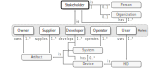
\includegraphics[scale=0.9]{figures/stakeholder}
  \caption{
    The stakeholder as either a person or organization, where each such stakeholder takes on one ore more distinct roles.
    The array of roles is not complete.
    \GlossaryHyperRef{hid}{HID} is an abbreviation for \GlossaryHyperRef{device-human-interface}{Human Interface Device}.
  }
  \label{fig:stakeholder}
\end{figure}

The roles occupied by a given stakeholder dictates what \GlossaryHyperRef{entity}{entities} that person or organization will interact with, as well as the nature of those interactions.
In Figure \ref{fig:stakeholder}, (1) \GlossaryHyperRef{owner}{owner}, (2) \GlossaryHyperRef{supplier}{supplier}, (3) \GlossaryHyperRef{developer}{developer}, (4) \GlossaryHyperRef{operator}{operator} and (5) \GlossaryHyperRef{user}{user} are named explicitly, but more roles are likely to be relevant, such as (6) \GlossaryHyperRef{acquirer}{acquirer} and (7) \GlossaryHyperRef{maintainer}{maintainer}, (8) \GlossaryHyperRef{builder}{builder}, (9) \GlossaryHyperRef{researcher}{researcher} and (10) \GlossaryHyperRef{architect}{architect}.
The listed ten names should be used rather than any synonyms when referring to these particular roles.
Please refer to the \hyperref[sec:glossary]{glossary} for their definitions.
If this document is read electronically, each role name can be clicked to be taken to its definition.

\subsection{Entity}
\label{sec:concepts:entity}

An \GlossaryHyperRef{entity}{entity} is an \GlossaryHyperRef{artifact}{artifact} that it \GlossaryHyperRef{identifiable}{identifiable}, which means that it can be distinguished from all other artifacts.
We use the word \textit{artifact} to refer to any object or thing, physical or intangible.
As depicted in Figure \ref{fig:entity}, this means that an entity always has an \GlossaryHyperRef{identity}{identity}.

\vfill

\begin{figure}[ht!]
  \centering
  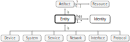
\includegraphics[scale=0.9]{figures/entity}
  \caption{
    The entity as an artifact with an identity.
    An entity or artifact may or may not be considered to be a \GlossaryHyperRef{resource}{resource}, in which case it is deemed to be valuable or useful from the perspective of a \GlossaryHyperRef{stakeholder}{stakeholder}.
    The array of artifacts with an \textit{is}-relation to \textit{Entity} is not complete.
    Other examples include \GlossaryHyperRef{cloud-local}{local clouds}, \GlossaryHyperRef{policy}{policies} and \GlossaryHyperRef{profile}{profiles}.
  }
  \label{fig:entity}
\end{figure}

Note that having an identity is not the same as being associated with an \GlossaryHyperRef{identifier}{identifier}, which is a name, number or other value referring to an entity.
It is enough that any such identifier is possible to produce for an artifact to count as an entity.
That being said, certain \GlossaryHyperRef{identification}{identification} requirements, perhaps related to security, performance or discoverability, may make it impractical to treat any other artifacts as entities than those with identifiers.

\subsection{Device}
\label{sec:concepts:device}

A \GlossaryHyperRef{device}{device} is a physical \GlossaryHyperRef{entity}{entity} with certain automation and compute \GlossaryHyperRef{capability-device}{capabilities}.
Examples of capabilities include moving robotic arms, reading from sensors, running \GlossaryHyperRef{software}{software}, and sending \GlossaryHyperRef{message}{messages}.
Every device must be capable of \GlossaryHyperRef{hosting-system}{\textit{hosting}} at least one \GlossaryHyperRef{system}{system}, which are \GlossaryHyperRef{communication}{communicating} \GlossaryHyperRef{instance-software}{software instances}.
Devices consist of \GlossaryHyperRef{component-hardware}{hardware components}.
While there are no limits to what such components can make up a device, each device must always have (1) \GlossaryHyperRef{unit-memory}{memory}, (2) \GlossaryHyperRef{unit-compute}{compute} and (3) \GlossaryHyperRef{interface-device}{interfacing} components, as shown in Figure \ref{fig:device}.

\vfill

\begin{figure}[ht!]
  \centering
  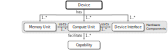
\includegraphics[scale=0.9]{figures/device}
  \caption{
    The device as a set of hardware components, each with zero or more automation or compute capabilities.
    Devices host \GlossaryHyperRef{component-software}{software components} using their compute units, even if not shown explicitly.
    Other examples of hardware components could be sensors, actuators, compute accelerators and batteries.
  }
  \label{fig:device}
\end{figure}

Every device must be able to host at least one system, or it is to be considered as being a hardware component.
While it may seem unintuitive to consider certain machines as components, such as large pumping complexes or vehicles with only manual controls, the \GlossaryHyperRef{framework-arrowhead}{Arrowhead framework} is meant to facilitate automation through the use of interconnected devices with compute capabilities.
If a machine cannot run software, making it able to host systems, that capability must be added before it can play a meaningful role in an \GlossaryHyperRef{arrowhead}{Arrowhead} context.
Consequently, machines without system hosting capabilities must either be considered as components or not be considered from the perspective of Arrowhead at all.

\newpage

\subsection{System}
\label{sec:concepts:system}

A \GlossaryHyperRef{system}{system} is an \GlossaryHyperRef{identifiable}{identifiable} \GlossaryHyperRef{instance-software}{software instance} that is \GlossaryHyperRef{hosting-system}{hosted} by a \GlossaryHyperRef{device}{device}.
As shown in Figure \ref{fig:system}, a system consists of \GlossaryHyperRef{component-software}{software components}.
Just as \GlossaryHyperRef{component-hardware}{hardware components}, software components can have various types of automation or compute \GlossaryHyperRef{capability-system}{capabilities}.
Every system should have the capability of \GlossaryHyperRef{consumer-service}{consuming services}, \GlossaryHyperRef{provider-service}{providing services}, or both.
If a given system can do neither, it must be referred to as an \GlossaryHyperRef{system-opaque}{\textit{opaque system}}.

\begin{figure}[ht!]
  \centering
  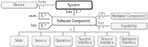
\includegraphics[scale=0.9]{figures/system}
  \caption{
    The system as a set of related software components, endowing a hosting device with new automation or compute capabilities.
    Other examples of software components could be operating systems, file systems, software libraries, programming language runtimes, databases and virtual machines.
  }
  \label{fig:system}
\end{figure}

Note that systems are not required to have any particular relationships to operating system processes, binary formats, virtual machines, and so on.
They may be \GlossaryHyperRef{implementation-software}{implemented} in any way deemed suitable.

\subsection{Service}
\label{sec:concepts:service}

A \GlossaryHyperRef{service}{service} is an \GlossaryHyperRef{identifiable}{identifiable} set of \GlossaryHyperRef{interface-service}{service interfaces} and \GlossaryHyperRef{operation-service}{operations}.
Each \textit{service interface} represents one way in which the service can receive and/or send \GlossaryHyperRef{message}{messages}, while each \textit{operation} represents one activity the \GlossaryHyperRef{system}{system} \GlossaryHyperRef{provider-service}{providing} the service can perform, if a \GlossaryHyperRef{message-valid}{valid} and \GlossaryHyperRef{message-permitted}{permitted} message is received.
As depicted in Figure \ref{fig:service}, service interfaces pass on, or \GlossaryHyperRef{routing-message}{route}, received messages to \GlossaryHyperRef{interface-operation}{operation interfaces}, which in turn may execute their associated operations with the messages as arguments.
Those operations may then send additional messages via the same or other operation interfaces, which will pass them on toward other operations.

\vfill

\begin{figure}[ht!]
  \centering
  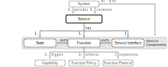
\includegraphics[scale=0.9]{figures/service}
  \caption{
    The service as a set of service interfaces and operations, making it possible for a providing system to offer the use of its capabilities to consuming systems via its service interfaces.
  }
  \label{fig:service}
\end{figure}

As all operations are \GlossaryHyperRef{component-software}{software components}, they may use any \GlossaryHyperRef{capability}{capabilities} of the devices and systems that host and provide them, respectively.
If capable of it, an operation may send any number of messages to other operations, with any kinds of delays or intervals, once it has been successfully consumed.
Messages can be sent within individual services, between services provided by the same system, between services provided by distinct systems hosted by the same device, or between services provided by systems residing on different devices, as described in Section \ref{sec:concepts:interface}.
When a service starts up and shuts down, it may be considered as if receiving an implicit message via an \textit{initialization} or \textit{termination} operation, respectively.
The messages to both of these operations may carry \GlossaryHyperRef{configuration}{configuration} \GlossaryHyperRef{data}{data} produced by and/or given to the system providing the service.

\subsection{System-of-Systems}
\label{sec:concepts:sos}

A \GlossaryHyperRef{system-of-systems}{system-of-systems} is a set of at least two \GlossaryHyperRef{system}{systems}, together facilitating one or more \GlossaryHyperRef{capability-system}{capabilities} none of the constituent systems could have on its own.
The facilitation of new capabilities is accomplished by the systems providing services and/or consuming each other's services.

While it may seem as if consuming services would hardly be enough for new capabilities to always emerge, it actually is the case.
For example, let us assume that a system has the capability of turning on and off a light.
That system also provides a service allowing for other systems to request that the light be turned on or off.
If a different system can successfully consume that service, it also gains the capability of turning on and off that particular light.
As a new system now may control that particular light, a new capability has emerged.

\subsection{Local Cloud}
\label{sec:concepts:local-cloud}

A \GlossaryHyperRef{cloud-local}{local cloud} is an \GlossaryHyperRef{identifiable}{identifiable} \GlossaryHyperRef{system-of-systems}{system-of-systems} able to execute given tasks through the use of a pool of \GlossaryHyperRef{resource}{resources}.
The resource pool of a local cloud could contain 3D-printers, autonomous unmanned vehicles, conventional servers, or anything else producing a value on demand.
As depicted in Figure \ref{fig:local-cloud}, the local cloud is distinct from other types of \GlossaryHyperRef{cloud}{clouds} by having at least one \GlossaryHyperRef{boundary-local}{local boundary} and one \GlossaryHyperRef{resource-local}{local resource}, which means that it is physically tied to a concrete location.
A local cloud could be engaged in manufacturing, repairs, heating, electricity distribution, workspace monitoring, drone fleet control, among many other possible kinds of physical activities.
A local cloud may be stationary or mobile.
A cloud that has no resources or boundaries tied to any particular physical locations should be referred to as a \GlossaryHyperRef{cloud-virtual}{\textit{virtual cloud}}.

\vfill

\begin{figure}[ht!]
  \centering
  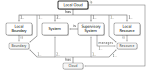
\includegraphics[scale=0.9]{figures/local-cloud}
  \caption{
    The local cloud as a regular cloud with at least one local boundary and one local resource.
  }
  \label{fig:local-cloud}
\end{figure}

That a local cloud has a boundary means that a distinction is being made between \GlossaryHyperRef{system}{systems} inside and outside the cloud.
A boundary being local means that the distinction is being made by a physical \GlossaryHyperRef{attribute}{attribute}, such as device location, type of device, or physical attachment to a certain \GlossaryHyperRef{entity}{entity}.
Boundaries may be protected, which means that measures are in place to guarantee security, safety, real-time characteristics, or other local cloud attributes.
The resources of a local cloud may be of any type, from virtual compute resources to physical drills or pumps.
A system managing a resource may be referred to as a \GlossaryHyperRef{system-supervisory}{\textit{supervisory system}}.

\subsection{System-of-Local-Clouds}
\label{sec:concepts:solc}

A \GlossaryHyperRef{system-of-local-clouds}{system-of-local-clouds} is two or more \GlossaryHyperRef{cloud-local}{local clouds} that \GlossaryHyperRef{consumer-service}{consume} each other's \GlossaryHyperRef{service}{services} to facilitate new \GlossaryHyperRef{capability-system}{capabilities}.
It is similar to the local cloud, with the exception of its \GlossaryHyperRef{subsystem}{subsystems} are \GlossaryHyperRef{cloud-local}{local clouds} instead of plain \GlossaryHyperRef{system}{systems}.
A system-of-local-clouds may have its own \GlossaryHyperRef{boundary-cloud}{boundaries} in addition to those of its constituent local clouds.
Those boundaries are formed by attributes shared by all the constituent local clouds, such as certificates issued by the same organization, or physical attachment to the same network bus.
A system-of-local-clouds cannot have resources beyond those of its constituent clouds, however.

\subsection{Network}
\label{sec:concepts:network}

A \GlossaryHyperRef{network}{network} is a set of two or more \GlossaryHyperRef{device-end}{end devices}, \GlossaryHyperRef{connection}{connected} via \GlossaryHyperRef{interface-network}{network interfaces} such that \GlossaryHyperRef{message}{messages} can pass between them.
As shown in Figure \ref{fig:network}, end devices may be \GlossaryHyperRef{interconnection}{interconnected} via \GlossaryHyperRef{device-intermediary}{intermediary devices}, examples of which could be routers, switches, hubs, busses and firewalls.
Any technology able to connect end devices is treated as facilitating networks, even if not typically associated with conventional networking methods.

\vfill

\begin{figure}[ht!]
  \centering
  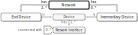
\includegraphics[scale=0.9]{figures/network}
  \caption{
    The network as a set of connected end devices, potentially interconnected via intermediary devices.
  }
  \label{fig:network}
\end{figure}

Messages can only pass between network interfaces if they are connected and their connection is \GlossaryHyperRef{connection-live}{\textit{live}}.

\subsection{Interface}
\label{sec:concepts:interface}

An \GlossaryHyperRef{interface}{interface} is an \GlossaryHyperRef{identifiable}{identifiable} \GlossaryHyperRef{boundary}{boundary} over which \GlossaryHyperRef{message}{messages} adhering to a supported \GlossaryHyperRef{protocol}{protocol} can cross, if those messages satisfy all \GlossaryHyperRef{policy}{policies} associated with that interface.
When considering \GlossaryHyperRef{service}{service} \GlossaryHyperRef{provision-service}{provision} and \GlossaryHyperRef{consumption-service}{consumption}, four types of interfaces become particularly relevant.
These are (1) \GlossaryHyperRef{interface-device}{device interfaces}, (2) \GlossaryHyperRef{interface-system}{system interfaces}, (3) \GlossaryHyperRef{interface-service}{service interfaces} and (4) \GlossaryHyperRef{interface-operation}{operation interfaces}, arranged as outlined in Figure \ref{fig:interface}.

\vfill

\begin{figure}[ht!]
  \centering
  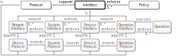
\includegraphics[scale=0.9]{figures/interface}
  \caption{
    The interface as a set of supported protocols and enforced policies.
    Devices, systems, services and operations have their own interface types, forming four stages through which messages can be passed.
  }
  \label{fig:interface}
\end{figure}

These four interface types form four stages, beginning with the device interface to the left.
Whenever any of these stages receives a message, it will either \textit{send} it leftwards or \textit{route} it rightwards, depending on whichever direction brings the message closest to the \GlossaryHyperRef{operation-service}{service operation} it targets.
If, for example, a message is targeting a service operation on a different system on the same device, it must be sent leftwards until it reaches the appropriate system interface, after which it can be routed rightwards.
Device interfaces send messages to other devices or to \GlossaryHyperRef{person}{persons}, depending on if they are \GlossaryHyperRef{interface-network}{network interfaces} or \GlossaryHyperRef{interface-human}{human interfaces}, respectively.
Operation interfaces do not route messages, but execute operations, as described in Section \ref{sec:concepts:service}.

Every interface only supports a limited set of protocols.
This means that passing messages between two interfaces requires that both support at least one common protocol.
If considering our four interface stages depicted in Figure \ref{fig:interface}, this means that a message can only pass between two adjacent stages if it adheres to a protocol supported by the right stage that is also an extension of a protocol supported by the left stage.
More details regarding protocols extending each other can be read in Section \ref{sec:concepts:protocol}.

\subsection{Protocol}
\label{sec:concepts:protocol}

A \GlossaryHyperRef{protocol}{protocol} is an \GlossaryHyperRef{identifiable}{identifiable} \GlossaryHyperRef{description}{description} of what \GlossaryHyperRef{message}{messages} may move between \GlossaryHyperRef{interface}{interfaces}.
A protocol is formulated as a set of \GlossaryHyperRef{type-message}{message types} and another set of \GlossaryHyperRef{type-state}{state types}.
Messages types determine what \GlossaryHyperRef{data}{data} valid messages must and may contain, while each state type dictates when certain messages are valid in relation to a certain \GlossaryHyperRef{state-protocol}{state}.
As shown in Figure \ref{fig:protocol}, a protocol may also be defined as an \GlossaryHyperRef{protocol-extensible}{extension} of another protocol, as well as be constrained by certain \GlossaryHyperRef{profile-protocol}{profiles} and \GlossaryHyperRef{encoding}{encodings}.

\begin{figure}[ht!]
  \centering
  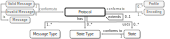
\includegraphics[scale=0.9]{figures/protocol}
  \caption{
    The protocol as set of message and state types, conforming to certain profiles and encodings.
  }
  \label{fig:protocol}
\end{figure}

Protocols must often extend each other to allow for messages to pass between interfaces of different types, such as the ones outlined in Section \ref{sec:concepts:interface}.
For example, the HTTP protocol \cite{fielding2014hypertext} is formulated as an extension of the TCP protocol \cite{postel1981transmission}, which is an extension of the IP protocol \cite{deering2017internet}, which can be an extension of the Ethernet protocol \cite{iso202188023}.
The HTTP protocol is, in fact, designed to be extended by such that ...

A \textit{profile} is a set of constraints added to every message of a protocol, defined only in terms of the contents of messages and the current protocol state.
Profiles can be used to specify how authorization tokens are to be included in messages, or demand that a certain message semantics be observed.
Adding a profile to a protocol not already conforming to it produces a new protocol.

\textit{Encodings} introduce \GlossaryHyperRef{system-type}{type systems} in which message payloads can be expressed.
If a protocol defines its messages without referring to an encoding, it is considered to have a \textit{custom} encoding.

%Each of these interface levels depend on the layer below it, with the exception of the device interface at the bottom.
%As each interface supports its own set of protocols, each interface layer must support a protocol that extends that of the below layer.
%A device interface may, for example, support the IP \cite{deering2017internet} protocol via Ethernet \cite{iso202188023}, a system interface the HTTP \cite{fielding2014hypertext} protocol via TCP \cite{postel1981transmission}, and a service interface a custom HTTP extension allowing for a target service operation to be specified.
%Note that the protocol at each layer may consist of multiple protocols extending each other, as in this example.
%A particular chain of protocols supported by a device, system or service is referred to as a \GlossaryHyperRef{stack-protocol}{\textit{protocol stack}}.
%The protocol stack of the system in the previous example would be Ethernet, IP, TCP and HTTP, from the bottom and up.

\subsection{Policy}
\label{sec:concepts:policy}

A \GlossaryHyperRef{policy}{policy} is an \GlossaryHyperRef{identifiable}{identifiable} set of \GlossaryHyperRef{constraint}{constraints}, useful for determining if given \GlossaryHyperRef{message}{messages} are acceptable or not, as depicted in Figure \ref{fig:policy}.
As messages are always meant to \GlossaryHyperRef{invocation-operation}{invoke operations}

that must be satisfied by a \GlossaryHyperRef{message}{message} for the activity associated with a certain \GlossaryHyperRef{operation-service}{service operation} to be permitted, 
A policy may use any of the \GlossaryHyperRef{capability-system}{capabilities}, or other provisions, of its system to determine if a given message is permitted.
Policies may be concerned with authorization, contracts, economic goals, and so on.
If a \GlossaryHyperRef{message}{message} \GlossaryHyperRef{invocation-operation}{invoking} a particular service operation fails to satisfy one or more of its policies, the sender of that message should be notified about what policies are being violated.

\begin{figure}[ht!]
  \centering
  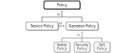
\includegraphics[scale=0.9]{figures/policy}
  \caption{
    The policy as a set of constraints.
    The types of constraints depicted are to be considered only as a limited set of possible examples.
    \GlossaryHyperRef{qos}{QoS} is an abbreviation for \GlossaryHyperRef{service-quality-of}{quality of service}.
  }
  \label{fig:policy}
\end{figure}

While policies are only explicitly associated with operations in this document, a derived work may choose to associate policies also with services, systems, system-of-systems and/or devices.
Such policies must be understood to apply to every operation made available by any such entity.
